%! suppress = MissingLabel


\chapter{Simulation Study}\label{ch:simulation-study}


\section{ParallelQueue Package}\label{sec:parallelqueue-package}
%======================================================================
In order to generate and study parallel queueing processes, few trivial options currently exist.
Moreover, while there exist some discrete event simulation (DES) frameworks which indeed focus on queueing networks, they currently tend not to permit the simultaneous study of asynchronous, redundancy-based schemes~\cite{noauthor_ciwpythonciw_nodate}.
In order to visualize and analyse the large class of queueing systems within this paradigm~\cite{shneer_large-scale_2020,cruise_stability_2020}, I introduced a novel module for Python which is currently available on PyPi: \textit{ParallelQueue} extending the DES package \textit{SimPy}.

The package currently allows for the studying of parallel systems with or without redundancy as well as with the option of allowing thresholds to be implemented in either case.
Moreover, the package allows one to specify any inter-arrival and service time distribution as well as their own \lstinline{Monitor}s, being a class which can gather data from the ongoing simulation to be distributed back to the user upon the completion of a simulation.
In particular, the \lstinline{Monitor}s are currently configured to collect data upon arrival, routing, and job completion as demonstrated by Figure~\ref{fig:API}.

Take Listing~\ref{lst:red} for example, which permits one to simulate a Redundancy(2) queueing system with 100 queues in parallel for 1000 units of time while returning the total queue counts over time (which are updated upon a change in queue count).
By merely calling \textit{totals.plot()} after importing \textit{Matplotlib}, Figure~\ref{fig:redpic} is easily retrieved.

\begin{lstlisting}[label={lst:red}, caption={Simulation of a redundancy system}, language={Python}, style={mystyle}]
#!/usr/bin/python3
from parallelqueue.base_models import RedundancyQueueSystem
from parallelqueue.monitors import TimeQueueSize
import random

sim = RedundancyQueueSystem(
                    maxTime=1000.0,parallelism=100, seed=1234,
                    d=2, Arrival=random.expovariate,
                    AArgs=9, Service=random.expovariate,
                    SArgs=0.08, Monitors = [TimeQueueSize])
# Note RedundancyQueueSystem is a ParallelQueueSystem wrapper
sim.RunSim()
totals = sim.MonitorOutput["TimeQueueSize"]
\end{lstlisting}

\begin{figure}
    \centering
    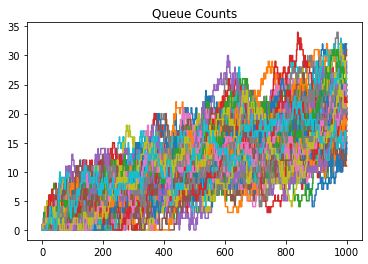
\includegraphics[scale=0.8]{redundancy}
    \caption{Queue size processes for $\text{Redundancy}(2)$}
    \label{fig:redpic}

    \medskip
\end{figure}

Remarkably, the simulation itself is performed speedily on consumer hardware despite the size of the system as demonstrated in Listing~\ref{lst:lstlisting2}.
\begin{lstlisting}[label={lst:lstlisting2},style=mystyle, caption={Runtime statistics using the master \textit{ParallelQueue} branch}]
CPU times: user 2.02 s, sys: 9.57 ms, total: 2.03 s
Wall time: 2.05 s
Intel i5-8250U (8) @ 3.400GHz
\end{lstlisting}


Altogether, this makes the package easy to parallelize with and thus to compare systems of different sizes
and with large running times.
While currently not implemented in any development branch of \textit{ParallelQueue}, the base Python package
\textit{multiprocessing} is used in throughout this paper when simulating for the same system across parameters.
In general, the main caveat when processing many models is that the storage of the simulation results can quickly begin
to consume storage;
when processing many models, it is therefore important to ensure that they are saved (e.g., using \textit{pickle}) and removed from
the local environment when doing analysis.

In terms of development, the models implemented in the \textit{base\_models} module use the framework established in Chapter~\ref{ch:model-specification}.
That is, in modelling redundancy, a hyperedge of sorts is generated whence the dispatcher
receives a job to be cloned.
This hyperedge then exists for the duration of time for which the replica class is in the system and is defined in such
a way that \textit{Monitor} class objects can interact with them in order to acquire data.
In Python, such a data structure can be implemented rather easily by employing the \textit{Dict} type which defines
a keyed set of values.
By keying based on the job arrivals (before cloning), a unique set of marks can be retrieved for the set by simply using
the \textit{Dict} object as a reference.

\begin{figure}
    \centering
    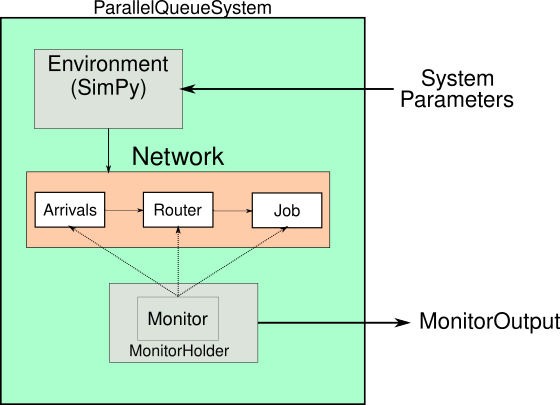
\includegraphics[scale=0.7]{pq}
    \caption{Overview of the \textit{ParallelQueue} API}
    \label{fig:API}
\end{figure}


\section{Results}\label{sec:results}

\subsection{Methodology}\label{subsec:methodology}
First, we examine each model in terms of their respective performance in $E(T)$, the expected time each job spends in the system.
As Figure~\ref{fig:img} shows, for a load $\rho \triangleq \frac{\lambda}{\mu} = 0.5$ by taking $\mu=1$ and $\lambda = 0.5$ (we will assume $\mu \equiv 1$ for the
rest of the simulations), Redundancy(2)) and Threshold(2,2) policies are rather alike with low loads as $N \rightarrow \infty$ in terms .
This is to be expected, of course, given that even such a low threshold is unlikely to be exceeded with the processors acting faster than arrivals on average.
Ignoring cancellation costs, this clearly demonstrates how utilizing otherwise dormant queues comes to benefit the system's performance.

\begin{figure}
    \centering
    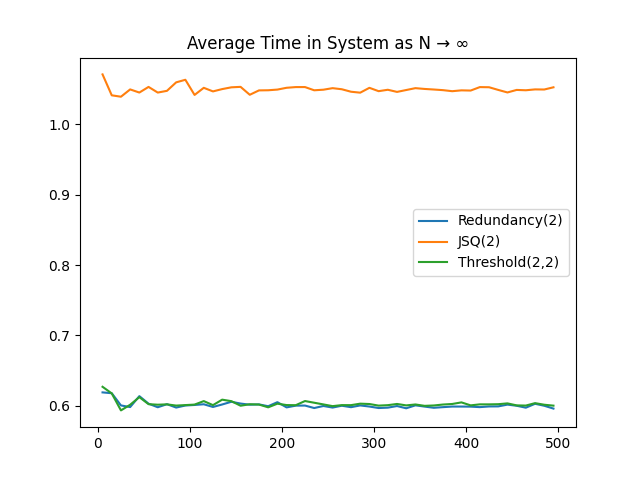
\includegraphics[width=0.7\linewidth]{compare_red_thr}
    \caption{Comparison of routing schemes: Values are averaged over 24 independent iterations each, running for $t=1000$}
    \label{fig:img}
\end{figure}

As shown in~\cite{gardner_redundancy-d_2017}, a Redundancy($d$) system is asymptotically stable if and only if $\rho < 1 $. Given that, in premise, Threshold($r,d$) models are more or less a superclass of Join-The-Shortest queue and Redundancy($d$) (trivially with rising $r$  implying no threshold exists and thus copies should always be made as in the case of Redundancy($d$)), it is perhaps most interesting to examine if threshold models are better able to handle high-load environments. Proving the superclass property in terms of redundancy is relatively easy and is done in Lemma~\ref{sup}. By contrast, after merely setting $r \equiv 0$, we get $ \mathcal{D}_{\text{Thresh(0,d)}} \overset{d}{=} \mathcal{D}_{\text{JSQ(d)}}$ by definition.
To prove the lemma, we first must introduce the concepts of stochastic domination and coupling as defined in~\cite{bramson_asymptotic_2012}.
\begin{definition}[Stochastic Domination]
    \\~\\
    $\mathbf{X}_{1}^{(N)}$ is said to dominate $\mathbf{X}_{2}^{(N)}$, using the notation $\leq_{st}$, when
    \[\mathbf{X}_{1}^{(N)}\leq_{st}\mathbf{X}_{2}^{(N)} \iff\# X_{1,i} \leq \# X_{2,i}  \quad \forall i \in [N] \quad P-a.s.\]
\end{definition}

\begin{definition}[Coupled Process]
    \label{coupled}
    \\~\\
    For stochastic processes $X_{t} \in \Pr(\Omega_{x}, \mathcal{F}_{x}, \mathcal{F}_{t,x})$ and $Y_{t} \in \Pr(\Omega_{y}, \mathcal{F}_{y}, \mathcal{F}_{t,y})$,
    $X_{t}$ and $Y_{t}$ are said to be coupled over the probability space $\Pr(\Omega, \mathcal{F}, \mathcal{F}_{t})$ if there exists
    $\hat X_{t}, \hat Y_{t} \in \Pr(\Omega, \mathcal{F}, \mathcal{F}_{t})$ such that $\hat X_{t} \overset{d}{=}X_{t}$ and $\hat Y_{t} \overset{d}{=}Y_{t}$.
\end{definition}

\begin{lemma}
    \label{sup}
    For $\mathbf{X}^{(N)}$ being a system of queues such that $\rho < 1$,
    \normalfont \[\mathcal{D}_{\text{Thresh}(r,d)}\mathbf(X^{(N)}) \overset{r \rightarrow \infty}{\rightsquigarrow} \mathcal{D}_{\text{Redundancy}(d)}\mathbf(X^{(N)}).\]
\end{lemma}
\textit{Proof}:

To show the sequence of routing algorithms to be convergent, we will construct a coupling in such a manner that $\forall r \in \mathbb{R}^{+}$, the system is stochastically dominated by another which is made to be finite~\cite{baccelli_elements_2003} .
To do so, for $\mathbf{X}_{1}^{(N)}$ under $\text{Thresh}(r,d)$, let us denote the first arrival as $T_{\xi_{1}}$, at which time it is the case that a selection set, $\nu \subset [N] $, is prescribed wherein there exists $\hat X \in \{X_{i}\}_{i \in \nu} $ such that $ \# (\hat X) > r $.
Thus, for  $ t \in [0,T_{\xi_{1}})$, we have $\mathcal{D}_{\text{Thresh}\mathit{(r,d)}}\mathbf(X^{(n)}) = \mathcal{D}_{\text{Redundancy}\mathit{(d)}}\mathbf(X^{(n)})$.
For clarity, let us now consider $\mathbf{Y}^{(N)}$ to be a copy of  $\mathbf{X}^{(N)}$ such that they are independent, identical in distribution and in terms of the marks of \textit{arrival process and job-size draws} along with the queues parsed (as was similarly done in~\cite{bramson_asymptotic_2012} via Lemma 4.1 using Definition~\ref{coupled}).
Effectively, the only difference being left between these copies is $r$ changing which queues receive clones and thus, too, the mark of queue-dependency.
At time $T_{\xi_{1}}$, we clearly have $\mathcal{D}_{\text{Redundancy}\mathit{(d)}}\mathbf(X^{(n)}) = \mathcal{D}_{\text{Thresh}\mathit{(r,d)}}\mathbf(Y^{(n)})$ due to there being no existing jobs for which the threshold would preclude cloning in the case of Thresh($r,d$).
As such, we also have $\mathcal{D}_{\text{Thresh}(r,d)}(Y^{(N)}(T_{\xi_{1}}))\leq_{st}\mathcal{D}_{\text{Redundancy}(d)}(X^{(N)}(T_{\xi_{1}}))$.

Now, assume $\rho < 1$, thereby giving us $ \# Y_{i}  < \infty \quad \forall t \in \mathbb{R}^{+}$ with probability 1~\cite{gardner_redundancy-d_2017}.
As such, we have that $\forall r \in \mathbb{R}^{+}$ there exists $ \xi_{1}(r) $ such that
\[P_{r}(\mathbf{X}^{(N)} (t) = \mathbf{Y}^{(N)}(t) |t \in [0,T_{\xi_{1}})) = 1\]
using the notation $P_{r}(A) := P(\mathcal{D}_{M(r)}(A))$, wherein $M$ denotes the routing algorithm of process $A$.
Note that $\xi_{1} (r)$ is monotone increasing in $r$.
Letting $r \rightarrow \infty \Rightarrow \xi_{1} \rightarrow \infty$, and so we then have $\mathbf{X}^{(N)}(t) =  \mathbf{Y}^{(N)}(t) \quad \forall t \in \mathbb{R}^{+}$ in terms of distribution (i.e., as the result holds $\forall t \in \mathbb{R}^{+}$ as $r\rightarrow \infty$), implying the required weak convergence from below for $\mathcal{D}$ in law over system  $\mathbf{X}^{(N)}(t)$.  \qed

In order to actually test the hypothesized results with respect to independence, we employ the joint Hilbert-Schmidt Independence Criterion (HSIC)~\cite{jointindep} to test the independence of queue counting processes $\{\#X_{n}(t)\}_{n \in [N]}$ in a Monte Carlo-styled
simulation consisting of $N_{\text{MC}}$ simulations for the queueing process $\mathbf{X}^{(N)}$.
\begin{definition}[HSIC Test for Two Processes]

    \label{hsichat}
    Following~\cite{nonstat}, for processes $X_{t}$ and $Y_{t}$ with common time domain $t \in T$, denote by $\kappa_{x}, \kappa_{y}$ the kernels which
    map each process to a separable reproducing kernel Hilbert space ($\mathcal{H}_{x}, \mathcal{H}_{y}$, respectively).
    Define HSIC to be the $\mathcal{H}_{x} \otimes \mathcal{H}_{y}$ norm of the form
    \[\text{HSIC}(\mathcal{H}_{x},\mathcal{H}_{y}) = \|\mu_{XY} - \mu_{X} \otimes \mu_{Y}\|^{2}_{\mathcal{H}_{x} \otimes \mathcal{H}_{y}},\]
    where $\mu_{Z}$ denotes a mean embedding of process $Z$ onto space $\mathcal{H}_{Z}$.
    \\~\\
    In order to test the hypotheses of
    \[H_{0}: P_{XY} = P_{X}P_{Y} \quad vs. \quad H_{a}: P_{XY} \not = P_{X}P_{Y},\]
    where $P_{Z}$ denotes the marginal distribution of $Z$,~\cite{nonstat} suggests a resampling procedure.
    Specifically, for any estimator of $\text{HSIC}(XY)$, ${H_{\text{HSIC}}}(XY)$, sample a common set of $N_{\text{time}}$ times, $\{\tau_{\ell}\}_{\ell \leq N_{\text{time}}} \subset T$, and calculate
    \[K :=\{H_{\text{HSIC}}(X_{(\{\tau_{N_{\text{time}}}\})}Y_{\gamma(\tau_{N_{\text{time}}})}))\}_{\gamma \in \Gamma},\]
    where $X_{(\{\tau_{N_{\text{time}}}\})}$ denotes $X_{t}$ restricted to the sampled times $\{\tau_{N_{\text{time}}}\}$ and $\Gamma$ is a set of permutations on these $N_{\text{time}}$ samples ordered such that $K_{i} \leq K_{i+1}$.
    After taking $c_{\alpha} :=  K_{(1-\alpha)N_{\text{time}}}$, the null hypothesis is rejected if $H_{\text{HSIC}}(XY) > c_{\alpha}$.
\end{definition}

%Specifically, we utilize an extension of HSIC testing for non -stationary processes described in~\cite{nonstat}, wherein for some common set of $N_{\text{time}}$ sampled times, $\{\tau_{\ell}\}_{ell \leq N_{\text{time}}}$,
Unlike the procedure utilized by~\cite{nonstat}, however, we adopt a modification described in~\cite{jointindep} to test for joint independence across $N$ processes.
While retaining the time sampling procedure of~\cite{nonstat}, we are instead concerned with testing upon the so-called $d\text{HSIC}$.

\begin{definition}[$d$HSIC]

    \label{dhsic}
    For a set of $d$ stochastic processes $\mathcal{X} = \{X_{i}\}_{i \leq d}$, define $d\text{HSIC}$ as:
    \[d\text{HSIC}(\mathcal{X}) := \|\mu_{\bigotimes_{i \leq d}(P_{X_{i}})} - \mu_{\{P_{X_{i}}\}_{i \leq d}}\|_{\bigotimes_{i \leq d}\mathcal{H}_{X_{i}}}.\]
\end{definition}

Much like the procedure described in Definition~\ref{hsichat}, an estimator and critical value can also be calculated in order to test for independence.
The particular means of estimation used in this research is outlined in Sections 4.1, 4.2, and B.5 of~\cite{jointindep} and is
implemented in the codebase used for our simulations as outlined in Appendix~\ref{sec:sic}.

\subsection{Simulation Results}\label{subsec:simulation-results}
Utilizing the procedure outlined in~\ref{subsec:methodology}, we test the following hypotheses:
\begin{align*}
    \label{set 2}
    H_{0}:& \text{ as } N\rightarrow \infty, \text{ queues in queueing system } \mathbf{X}_{t}^{(N)} \text{ become jointly independent,}  \\
    H_{a}:& \text{ as } N\rightarrow \infty, \text{ queues in queueing system } \mathbf{X}_{t}^{(N)} \text{ do not become jointly independent.}
\end{align*}
Moreover, we are also interested in the case of $t \rightarrow \infty$ and thus also analyze the hypotheses:
\begin{align*}
    \label{set 1}
    H_{0}:& \text{ as } t\rightarrow \infty, \text{ queues in queueing system } \mathbf{X}_{t}^{(N)} \text{ become jointly independent,}  \\
    H_{a}:& \text{ as } t\rightarrow \infty, \text{ queues in queueing system } \mathbf{X}_{t}^{(N)} \text{ do not become jointly independent.}
\end{align*}

Altogether, these hypotheses comprise the behaviour expected of the system outlined in Figure~\ref{fig:1} for the limits of $\mathbf{X}^{(N)}(t)$
in terms of $t$ and $N$, respectively, according to Conjecture~\ref{conj}.

To test the first hypothesis, we calculate $d$HSIC under the chi square kernel at $\alpha = 0.1$ across $N \in \{5, 25, 50, 100, 500\}$
for time samples $\{\tau_{i} | \tau_{i} \sim U[i,i-1]\}_{0 < i \leq 100}$ where 100 is the simulation time-length.
Moreover, we test across varying $\rho \in \{0.8, 0.9, 0.99\}$ while keeping $\mu \equiv 1$.
As such, we have $\rho \overset{\Delta}= \frac{d\lambda}{N\mu} \iff \lambda = \frac{N \rho}{d}$ for each simulated system.
Simulations are run for 20 independent seeds at each $N\times\rho$ combination while each test is resampled $500$ times, being the maximum suggested in~\cite{jointindep}.
In all, as Table~\ref{tab:reg} summarizes, the hypothesis was rejected only for values of $N = 2, \rho \in \{0.9,0.99\}$.
It is noteworthy that JSQ($d$) of course also exhibits this property~\cite{bramson_asymptotic_2012}.
\begin{table}
    \centering
    \caption{$d$HSIC for varying $N$}
    \label{tab:reg}
    \begin{tabular}{|c|c|c|c|}
        \hline
        $\rho$ & $N$ & $r$ & $\hat p(H_{a})$ \\
        \hline
        \hline
        & 5   & 1   & 0.089 *         \\
        & 50  & 1   & 0.198           \\
        & 100 & 1   & 1.0             \\
        & 500 & 1   & 0.109           \\
        0.8    & 5   & 2   & 0.921           \\
        & 50  & 2   & 0.228           \\
        & 100 & 2   & 0.02 **         \\
        & 500 & 2   & 0.129           \\
        \hline
        & 5   & 1   & 0.089 *         \\
        & 50  & 1   & 0.891           \\
        & 100 & 1   & 0.693           \\
        & 500 & 1   & 0.861           \\
        0.9    & 5   & 2   & 1.0             \\
        & 50  & 2   & 0.178           \\
        & 100 & 2   & 0.109           \\
        & 500 & 2   & 0.634           \\
        \hline

        & 5   & 1   & 0.782           \\
        & 50  & 1   & 0.01 ***        \\
        & 100 & 1   & 0.386           \\
        & 500 & 1   & 0.347           \\
        0.99   & 5   & 2   & 0.406           \\
        & 50  & 2   & 0.327           \\
        & 100 & 2   & 0.485           \\
        & 500 & 2   & 0.475           \\
        \hline


    \end{tabular}

    \begin{tabular}{p{10cm}}
        \textit{Note:} * $\hat{p}(H_{a}) < 0.1$, ** $\hat{p}(H_{a}) < 0.05$, *** $\hat{p}(H_{a}) < 0.01$
        \\
        Data are drawn from 20 simulations run for each $N$.
    \end{tabular}
\end{table}

Indeed, it is apparent from Table~\ref{tab:reg} that the highest tested value consistently results in a failure to reject
the null hypothesis.
Interestingly, $N=2$ also prevented rejection of the hypothesis, however this might instead point to
the choice of kernel being inappropriate.
While beyond the scope of this project, utilization of $(\Lambda,\lambda)$ exchangeability
rather than full exchangeability might provide a more appropriate means of assessing independence.

Carrying on to the case of $t \rightarrow \infty$, we perform the same analysis but change the sampled times to
$\{\tau_{i} | \tau_{i} \sim U[i,i-1]\}_{900 \leq i \leq 1000}$.
By doing so, we restrict ourselves to a domain wherein the process is sufficiently burnt-in and thus likely approaching stationarity.
As summarized in Table~\ref{tab:longtime}, we see a similar pattern as in our prior testing which is, once again, indicative
of what would be expected under the conjecture.
$N=2$ is included in the results, however, as varying $r$ resulted in rejecting the hypothesis of independence only in the case where $r=1$ for the sampled times.
\begin{table}
    \centering
    \caption{$d$HSIC test for large $t$}
    \label{tab:longtime}
    \begin{tabular}{|c|c|c|c|}
\hline
$\rho$ & $N$ & $r$ & $\hat p(H_{a})$ \\
\hline
\hline
 & 2 & 1 & 0.000 *** \\
 & 5 & 1 & 0.549  \\
 & 50 & 1 & 0.743  \\
 & 100 & 1 & 0.443  \\
 & 500 & 1 & 0.741  \\
0.8 & 2 & 2 & 0.521  \\
 & 5 & 2 & 0.826  \\
 & 50 & 2 & 0.493  \\
 & 100 & 2 & 0.567  \\
 & 500 & 2 & 0.623  \\
\hline
 & 2 & 1 & 0.000 *** \\
 & 5 & 1 & 0.345  \\
 & 50 & 1 & 0.389  \\
 & 100 & 1 & 0.505  \\
 & 500 & 1 & 0.77  \\
0.9 & 2 & 2 & 0.485  \\
 & 5 & 2 & 0.948  \\
 & 50 & 2 & 0.409  \\
 & 100 & 2 & 0.13  \\
 & 500 & 2 & 0.405  \\
\hline
 & 2 & 1 & 0.000 *** \\
 & 5 & 1 & 0.275  \\
 & 50 & 1 & 0.938  \\
 & 100 & 1 & 0.423  \\
 & 500 & 1 & 0.525  \\
0.99 & 2 & 2 & 0.535  \\
 & 5 & 2 & 0.639  \\
 & 50 & 2 & 0.862  \\
 & 100 & 2 & 0.25  \\
 & 500 & 2 & 0.946  \\
        \hline

    \end{tabular}

    \begin{tabular}{p{10cm}}
        \textit{Note:} * $\hat{p}(H_{a}) < 0.1$, ** $\hat{p}(H_{a}) < 0.05$, *** $\hat{p}(H_{a}) < 0.01$
        \\
        Data are drawn from 20 simulations run for each $N$.
    \end{tabular}
\end{table}

Lastly, to test whether the system becomes asymptotically deterministic and reaches a fixed point, we concern ourselves with the hypotheses of:
\begin{align*}
    \label{chi 1}
    H_{0} :& \text{ }\mathbf{X}^{(N)}_{t} \overset{N,t \rightarrow \infty}{\rightarrow} \boldsymbol{\pi} \text{, a process which is degenerate in law,}  \\
    H_{a} :& \text{ }\mathbf{X}^{(N)}_{t} \overset{N,t \rightarrow \infty}{\not \rightarrow} \boldsymbol{\pi} \text{, a process which is degenerate in law.}
\end{align*}
We proceed in assessing the model by means of simulating a system at $N=500$ across $\rho \in \{0.8, 0.9 ,0.99\}$ and $r \in \{1,2\}$ for sampled times drawn from a uniform grid with a step size of $0.25$.
After $20$ repetitions, we average the size of each queue at each sampled time across each run.
From there, we calculate the autocorrelation function (ACF) for the average queue size at each combination of parameters, for which results are summarized in Figure~\ref{fig:autocor}.

\begin{figure}
    \centering
    \begin{tabular}{ccc}
        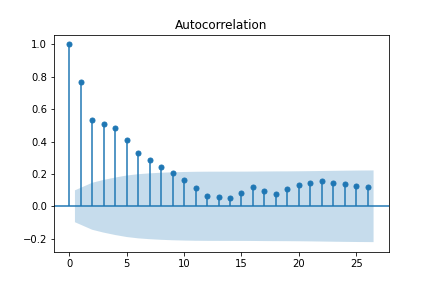
\includegraphics[width=50mm]{autocor/1_0_0.8_1614784150.46764}   & 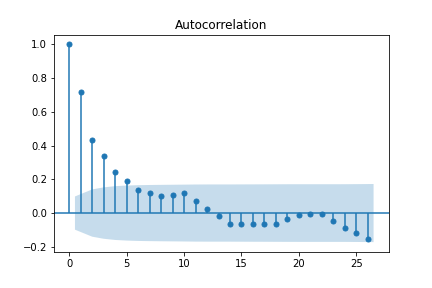
\includegraphics[width=50mm]{autocor/1_0_0.9_1614789195.7596514}
        & 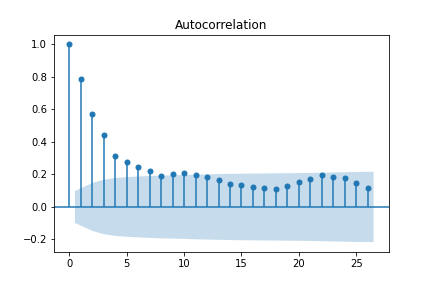
\includegraphics[width=50mm]{autocor/1_0_0.99_1614794552.4804938}\\
        (a) $r = 1, \rho = 0.8$                                          & (b) $r = 1, \rho = 0.9$                                          & (c) $r = 1, \rho = 0.99$ \\[6pt]
        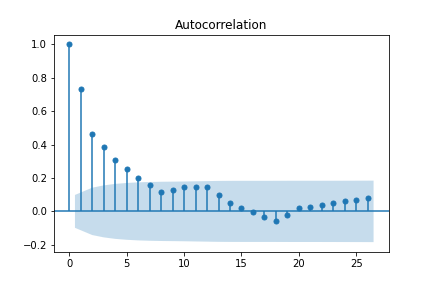
\includegraphics[width=50mm]{autocor/2_0_0.8_1614786651.7051768} & 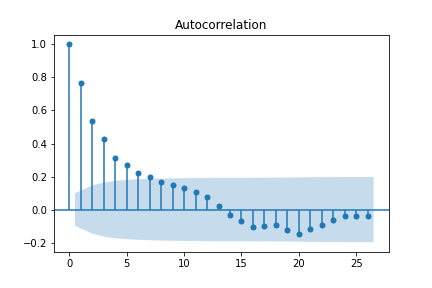
\includegraphics[width=50mm]{autocor/2_0_0.9_1614791739.9236946}
        & 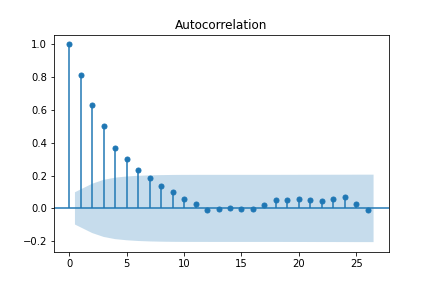
\includegraphics[width=50mm]{autocor/2_0_0.99_1614797400.487133}\\
        (c) $r = 2, \rho = 0.8$                                          & (d) $r = 2, \rho = 0.9$                                          & (e) $r = 2, \rho = 0.99$ \\[6pt]
    \end{tabular}
    \caption{Autocorrelations of $E(\#X_{n}(t))$ at $N = 500, t \in [900,1000]$ for varying $\rho, r$}
    \label{fig:autocor}
\end{figure}

At $\alpha = 0.05$, we observe that a statistically significant degree of serial dependence exists for lags near each tested point.
Inspection of the graphs reveal that, at such lags, autocorrelations are positive and decreasing in strength, as would be expected in a system having reached a fixed point.